\documentclass{article}
\usepackage{amsmath,amssymb,amsthm,latexsym,paralist,url}
\usepackage[margin=1in]{geometry}
\usepackage{tikz}
\usetikzlibrary{arrows,automata}

\theoremstyle{definition}
\newtheorem{problem}{Problem}
\newtheorem*{solution}{Solution}
\newtheorem*{resources}{Resources}


\newcommand{\honor}{\noindent \textbf{Aggie Honor Statement: }On my honor as an Aggie, I have neither
  given nor received any unauthorized aid on any portion of the academic work included in this assignment.
}

 
\newcommand{\checklist}{\noindent\textbf{Checklist:}
Did you...
\begin{compactenum}
\item abide by the Aggie Honor Code?
\item solve all problems?
\item start a new page for each problem?
\item show your work clearly?
\item type your solution?
\item submit a PDF to eCampus?
\end{compactenum}
}

\newcommand{\problemset}[1]{\begin{center}\textbf{Problem Set #1}\end{center}}
\newcommand{\duedate}[1]{\begin{quote}\textbf{Due: #1} on eCampus (\url{ecampus.tamu.edu}). \\You must show your work in order to recieve credit.\end{quote}}
\newcommand{\mysectionnumber}[0]{503}

\title{CSCE 222: Discrete Structures for Computing\\Section \mysectionnumber\\Fall 2016}
\author{Joseph Martinsen}

\begin{document}

\maketitle

\problemset{9}

\duedate{30 October 2016 (Sunday) before 11:59 p.m.}

\bigskip

% Regular Expressions
\begin{problem} (25 points)\\
\begin{enumerate}
\item Build a finite-state automaton that accepts the language $1^*0(1\cup01^*0)^*$.  Give an English description of the language (your description should be about 10 words long, of which the first 5 are \textit{the set of strings containing}).
\item Build a finite state automaton that recognizes the set of strings that end in 11 and do not contain 00. Convert this finite-state automaton into an equivalent regular expression.

\end{enumerate}
\end{problem}

\begin{solution}\ \\
  \begin{enumerate}
    \item The set of strings containing bitstrings 10, 0010, or 0
    \begin{center}
      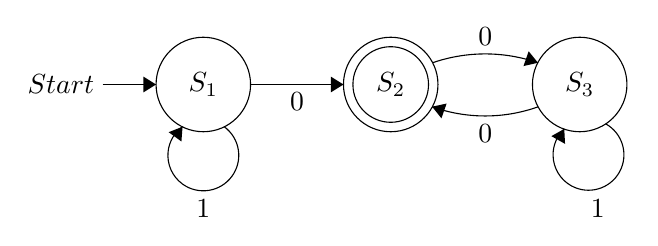
\begin{tikzpicture}[scale=0.2]
        \tikzstyle{every node}+=[inner sep=0pt]
        \draw [black] (12.3,-28.5) circle (3);
        \draw (12.3,-28.5) node {$S_1$};
        \draw [black] (24.2,-28.5) circle (3);
        \draw (24.2,-28.5) node {$S_2$};
        \draw [black] (24.2,-28.5) circle (2.4);
        \draw [black] (36.2,-28.5) circle (3);
        \draw (36.2,-28.5) node {$S_3$};
        \draw [black] (5.9,-28.5) -- (9.3,-28.5);
        \draw (5.4,-28.5) node [left] {$Start$};
        \fill [black] (9.3,-28.5) -- (8.5,-28) -- (8.5,-29);
        \draw [black] (26.852,-27.121) arc (109.08499:70.91501:10.239);
        \fill [black] (33.55,-27.12) -- (32.96,-26.39) -- (32.63,-27.33);
        \draw (30.2,-26.06) node [above] {$0$};
        \draw [black] (15.3,-28.5) -- (21.2,-28.5);
        \fill [black] (21.2,-28.5) -- (20.4,-28) -- (20.4,-29);
        \draw (18.25,-29) node [below] {$0$};
        \draw [black] (37.845,-30.995) arc (61.12502:-226.87498:2.25);
        \draw (37.35,-35.8) node [below] {$1$};
        \fill [black] (35.22,-31.32) -- (34.4,-31.78) -- (35.27,-32.27);
        \draw [black] (33.567,-29.915) arc (-70.33511:-109.66489:10.006);
        \fill [black] (26.83,-29.91) -- (27.42,-30.65) -- (27.75,-29.71);
        \draw (30.2,-31) node [below] {$0$};
        \draw [black] (13.623,-31.18) arc (54:-234:2.25);
        \draw (12.3,-35.75) node [below] {$1$};
        \fill [black] (10.98,-31.18) -- (10.1,-31.53) -- (10.91,-32.12);
      \end{tikzpicture}
    \end{center}
    
    \item \ \\
      \begin{center}
          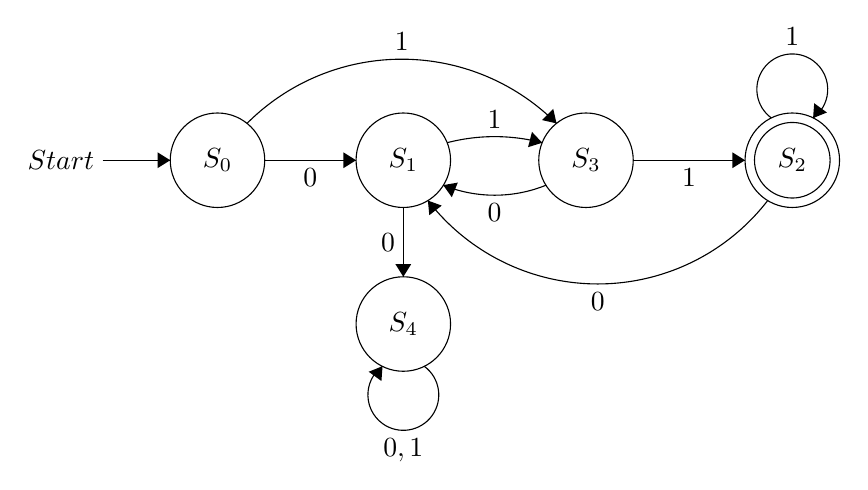
\begin{tikzpicture}[scale=0.2]
            \tikzstyle{every node}+=[inner sep=0pt]
            \draw [black] (13.8,-28.1) circle (3);
            \draw (13.8,-28.1) node {$S_0$};
            \draw [black] (25.6,-28.1) circle (3);
            \draw (25.6,-28.1) node {$S_1$};
            \draw [black] (50.3,-28.1) circle (3);
            \draw (50.3,-28.1) node {$S_2$};
            \draw [black] (50.3,-28.1) circle (2.4);
            \draw [black] (37.2,-28.1) circle (3);
            \draw (37.2,-28.1) node {$S_3$};
            \draw [black] (25.6,-38.5) circle (3);
            \draw (25.6,-38.5) node {$S_4$};
            \draw [black] (6.5,-28.1) -- (10.8,-28.1);
            \draw (6,-28.1) node [left] {$Start$};
            \fill [black] (10.8,-28.1) -- (10,-27.6) -- (10,-28.6);
            \draw [black] (15.672,-25.764) arc (135.09717:44.90283:13.875);
            \fill [black] (35.33,-25.76) -- (35.12,-24.84) -- (34.41,-25.55);
            \draw (25.5,-21.18) node [above] {$1$};
            \draw [black] (40.2,-28.1) -- (47.3,-28.1);
            \fill [black] (47.3,-28.1) -- (46.5,-27.6) -- (46.5,-28.6);
            \draw (43.75,-28.6) node [below] {$1$};
            \draw [black] (48.977,-25.42) arc (234:-54:2.25);
            \draw (50.3,-20.85) node [above] {$1$};
            \fill [black] (51.62,-25.42) -- (52.5,-25.07) -- (51.69,-24.48);
            \draw [black] (16.8,-28.1) -- (22.6,-28.1);
            \fill [black] (22.6,-28.1) -- (21.8,-27.6) -- (21.8,-28.6);
            \draw (19.7,-28.6) node [below] {$0$};
            \draw [black] (28.378,-26.988) arc (104.63673:75.36327:11.96);
            \fill [black] (34.42,-26.99) -- (33.77,-26.3) -- (33.52,-27.27);
            \draw (31.4,-26.1) node [above] {$1$};
            \draw [black] (34.669,-29.682) arc (-67.89017:-112.10983:8.684);
            \fill [black] (28.13,-29.68) -- (28.68,-30.45) -- (29.06,-29.52);
            \draw (31.4,-30.82) node [below] {$0$};
            \draw [black] (48.741,-30.656) arc (-37.68609:-142.31391:13.636);
            \fill [black] (27.16,-30.66) -- (27.25,-31.59) -- (28.04,-30.98);
            \draw (37.95,-36.46) node [below] {$0$};
            \draw [black] (25.6,-31.1) -- (25.6,-35.5);
            \fill [black] (25.6,-35.5) -- (26.1,-34.7) -- (25.1,-34.7);
            \draw (25.1,-33.3) node [left] {$0$};
            \draw [black] (26.923,-41.18) arc (54:-234:2.25);
            \draw (25.6,-45.75) node [below] {$0,1$};
            \fill [black] (24.28,-41.18) -- (23.4,-41.53) -- (24.21,-42.12);
          \end{tikzpicture}
        \end{center}
        \newpage
        \begin{align*}
          \text{Regular Expression: } (1 + (01)^*)(01)^*(1 + \lambda)^*
        \end{align*}
  \end{enumerate}
\end{solution}

% Turing Machines
\begin{problem} (25 points)\\
Construct a Turing machine that recognizes the set $\{0^{2n}1^n \mid n\geq 0\}$.  The Turing machine starts with the input on the tape and the head over the leftmost symbol of the input.  The symbols to the left of the input are blanks out to infinity, as are the symbols to the right of the input.  If the string is accepted, the machine should halt with 1 on the tape (the rest of the tape should be blank).  If the string is rejected, the machine should halt with 0 on the tape.\\
\textit{Note: this is not an easy task, it will take you several revisions to get it right, do not get discouraged.}
\end{problem}

\begin{solution}\ \\

\end{solution}

\newpage

% Relations
\begin{problem} (25 points)\\
For each relation on the set of all people, determine whether it is an equivalence realtion.  For each relation that is not an equivalence relation, determine which properties of an equivalence relation it lacks.  Your answers are not complete unless you include the definition of each property.
\begin{enumerate}
\item $\{(a,b) \mid a \text{ and } b \text{ are the same age }\}$
\item $\{(a,b) \mid a \text{ and } b \text{ have the same parents }\}$
\item $\{(a,b) \mid a \text{ and } b \text{ share a common parent }\}$
\item $\{(a,b) \mid a \text{ and } b \text{ have met }\}$
\item $\{(a,b) \mid a \text{ and } b \text{ speak a common language }\}$
\end{enumerate}
\end{problem}

\begin{solution}\ \\

\end{solution}

\newpage

% Relations
\begin{problem} (25 points)\\
Which of these are partially ordered sets?  For each relation whichis not a partial ordering, determine which properties of a partial ordering the relation lacks. Your answers are not complete unless you include the definition of each property.
\begin{enumerate}
\item $(\mathbb{R},=)$
\item $(\mathbb{R},\leq)$
\item $(\mathbb{R},>)$
\item $(\mathbb{R},\neq)$
\item $(\cal{P}(\mathbb{Z}),\subseteq)$, where $\cal{P}(\cdot)$ is the powerset.
\end{enumerate}
\end{problem}

\begin{solution}\ \\

\end{solution}

\bigskip
\honor

\bigskip
\checklist
\end{document}
